\documentclass{beamer}

\usepackage{graphicx}
\usepackage{bookmark}
\usepackage[sfdefault,light]{FiraSans}
\usepackage[british]{datetime2}
\usepackage{textcomp}
\usetheme{default}
\setbeamertemplate{navigation symbols}{} % No navigation symbols
\setbeamercolor{alerted text}{fg=blue!80!green!159!}
\setbeamercolor{frame title}{fg=blue!80!green!159!}
\setbeamercolor{title}{fg=blue!80!green!159!}
\setbeamercolor{subtitle}{fg=blue!80!green!159!}

%BLACK THEME (Remember to change the logos to _neg)
% \usecolortheme[named=white]{structure} % White titles and such
% \setbeamercolor{normal text}{fg=white} % White text
% \setbeamercolor{background canvas}{bg=black} % Black background

\makeatletter
\setbeamertemplate{footline}
{
  \leavevmode%
  \hbox{%
  \begin{beamercolorbox}[wd=.15\paperwidth,ht=2.25ex,dp=1ex,center]{institute in head/foot}%
    \usebeamerfont{title in head/foot}%
    \raisebox{-0.15cm}{
\includegraphics[width=1cm]{logo_ntnu_u-slagord.pdf}}
  \end{beamercolorbox}%
  \begin{beamercolorbox}[wd=.6\paperwidth,ht=2.25ex,dp=1ex,center]{institute in head/foot}%
    \usebeamerfont{title in head/foot}%
    \insertsection
  \end{beamercolorbox}%
  \begin{beamercolorbox}[wd=.15\paperwidth,ht=2.25ex,dp=1ex,center]{institute in head/foot}%
    \usebeamerfont{title in head/foot}%
    \insertshorttitle
  \end{beamercolorbox}%
  \begin{beamercolorbox}[wd=.1\paperwidth,ht=2.25ex,dp=1ex,right]{institute in head/foot}%
    \usebeamerfont{title in head/foot} 
    \insertframenumber{} / \inserttotalframenumber\hspace*{2ex} 
  \end{beamercolorbox}}%
}
\makeatother

%----------------------------------------------------------------------------------------
%	TITLE PAGE
%----------------------------------------------------------------------------------------

\title[POL2012]{POL2012: Theories and Models in Political Economy}
\subtitle{Introduction and Economic Systems}

\author[Wishman]{Marius Swane Wishman} % Your name
\date[August 2019]{\today} % Date
\institute{Department of Sociology and Political Science}

%\setbeamertemplate{background}{\includegraphics[width=\paperwidth]{Title.png}}

\begin{document}

\begin{frame}[plain]
\titlepage % Print the title page as the first slide
\centering % Comment out if second logo

\includegraphics[width=5cm]{logo_ntnu_u-slagord.pdf}
%\hspace{0.5cm} 
\includegraphics[width=5cm]{logo_ntnu_u-slagord.pdf} % Second logo ?
\end{frame}


\section{Introduction} % Sections can be created in order to organize your presentation into discrete blocks, all sections and subsections are automatically printed in the table of contents as an overview of the talk
%------------------------------------------------


\begin{frame}{Practical Info}

    \begin{itemize}[<+- | alert@+>]
        \item Build up of the course
        \item Hand-ins and seminars
        \item Term Paper
         \begin{itemize}[<+- | alert@+>]
            \item Pass/No Pass
            \item Based on extra curriculum sources
            \item Academic standards
            \item Deadline: Late October
        \end{itemize}
        \item Exam
        \begin{itemize}[<+- | alert@+>]
            \item 29th November
            \item 4 hour written exam
        \end{itemize}
    \end{itemize}

\end{frame}

\section{Fundamentals}

\begin{frame}{What is ``Political Economy"?}
\begin{itemize}[<+- | alert@+>]
    \item ``Most  commonly refers to interdisciplinary studies drawing upon economics, sociology, and political science in explaining how political institutions, the political environment, and the economic system - capitalist, socialist, or mixed - influence each other."\\
    - Weingast \& Wittman (2008)
\end{itemize}{}
\end{frame}{}

\begin{frame}{Relevance of Political Economy}
\begin{itemize}[<+- | alert@+>]
	\item Economic orthodoxy
	\item The role of markets
	\item The role of government
	\item Economy as self-equilibriating
	\item Growth, the default state
\end{itemize}
\end{frame}

\begin{frame}{Relevance of Political Economy}
\begin{itemize}[<+- | alert@+>]
	\item Financial crises
	\item Climate change
	\item Rising inequality
	\item Stagnating growth
\end{itemize}
\end{frame}

\begin{frame}{What are ``Theories and Models"?}
\begin{itemize}[<+- | alert@+>]
	\item Theory
	\item A set of logical arguments about causality
	\item What is not theory? 
	   \begin{itemize}[<+- | alert@+>]
            \item Literature
            \item Empirics
            \item Paradigms
            \item Models
        \end{itemize}
\end{itemize}
\end{frame}

\begin{frame}{Example -- is this theory?} 

	``Countries with better ``institutions," more secure property rights,
	and less distortionary policies will invest more in physical and human
	capital, and will use these factors more efficiently to achieve a
	greater level of income (e.g., Douglass C. North and Robert P. Thomas,
	1973; Eric L. Jones, 1981; North, 1981). This view receives some support
	from cross-country correlations between measures of property rights and
	economic development (e.g., Stephen Knack and Philip Keefer, 1995; Paulo
	Mauro, 1995; Robert E. Hall and Charles I. Jones, 1999; Dani Rodrik,
	1999), and from a few micro studies that investigate the relationship
between property rights and investment or output (e.g., Timothy Besley, 1995;
Christopher Mazingo, 1999; Johnson et al., 1999)." \end{frame}{}

\begin{frame}{Example -- is this theory?} 

	``Colonies where Europeans faced higher mortality rates are today
substantially poorer than colonies that were healthy for Europeans. Our theory
is that this relationship reflects the effect of settler mortality working
through the institutions brought by Europeans." \end{frame}

\begin{frame}{Theory}

    \begin{itemize}[<+- | alert@+>]
	
		\item Arriving at hypotheses
		\item Answering the ``why" of a causal claim
			(hypothesis)
	
	\end{itemize}

\end{frame}

\begin{frame}{Theory}

	\begin{figure}[!htb]
		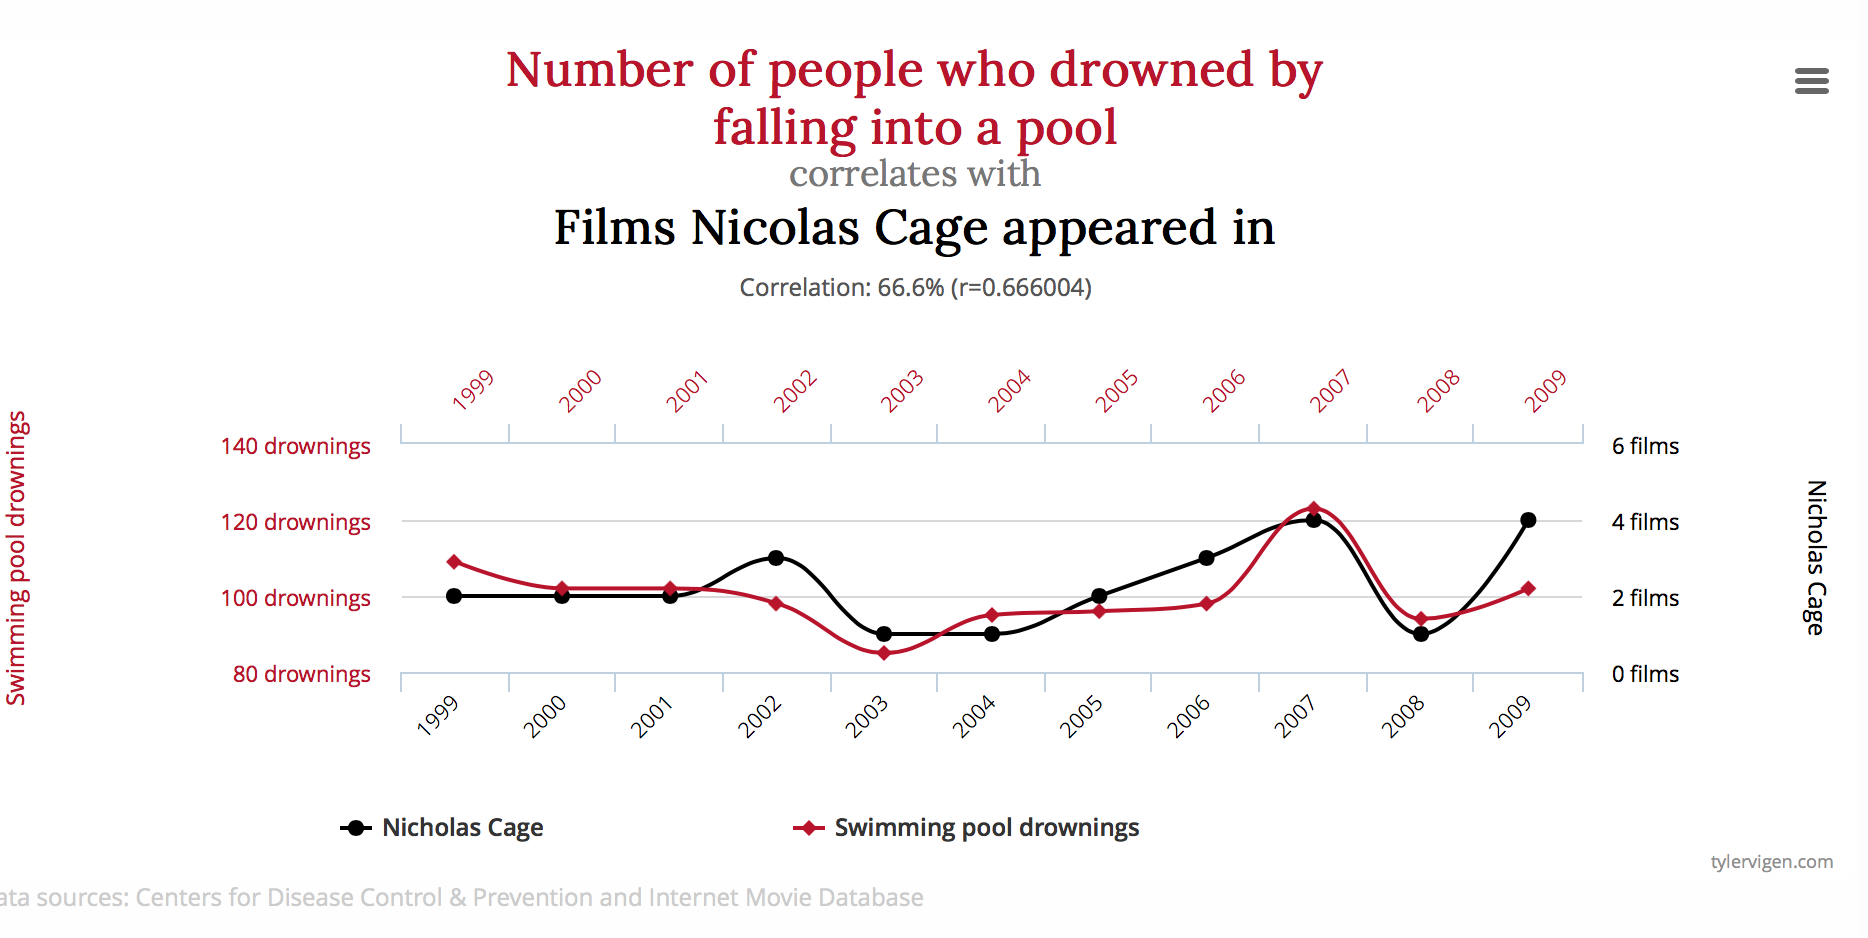
\includegraphics[width=\textwidth,keepaspectratio]{../img/correlationCausation.png}
	\end{figure}
	
\end{frame}

\begin{frame}{Theory}

	\begin{figure}[!htb]
		
\includegraphics[width=\textwidth,keepaspectratio]{../img/coincidence.jpeg}
	\end{figure}
	
\end{frame}

\begin{frame}{Theory}

\begin{itemize}[<+- | alert@+>]

	\item Theory 1: Nicholas Cage is a great actor (empirical statement) and
		his movies often involve swimming/drowning in pools (empirical
		statement).  (because) Any great actor wants his/hers movies to
		be realistic and so... (``A set of logical arguments about
		causality")

	\item Theory 2: Nicholas Cage is a terrible actor (empirical statement).
		So terrible in fact, that people become acutely suicidal
		(logical argument), the statistics on pool drownings is picking
		up part of this effect.

\end{itemize}

\end{frame}

\begin{frame}{Models}
    What is a model?
\end{frame}

\begin{frame}{Models}
    \begin{itemize}[<+- | alert@+>]

        \item Settler mortality \textrightarrow Type of settlement
        \textrightarrow Early institutions \textrightarrow Current institutions
        \textrightarrow Current economic performance

        \item \begin{equation}
            log Y_{i}=\alpha+\beta_{i}X_{i}+\epsilon_{i}
        \end{equation}

	\item Simplified version of a causal relationship 

    \end{itemize}
\end{frame}{}

\end{document} 

